\documentclass[10pt,a4paper]{scrartcl}
\PassOptionsToPackage{table}{xcolor}
\usepackage[utf8]{inputenc}
\usepackage[T1]{fontenc}
\usepackage[ngerman]{babel}
\usepackage{microtype, multicol, marginnote, bera, parskip}
\usepackage{listings, amsmath, amssymb, graphicx, tikz, epic}
\usepackage{stmaryrd} %for lightning arrow
\usepackage{pstricks, pst-node, pst-tree, pdflscape}
\usepackage[babel=true]{csquotes}
\usepackage{placeins}
\tolerance=2000
\setcounter{secnumdepth}{0}
\usepackage[inner=2cm,outer=2cm,top=1.5cm,bottom=1.5cm,includeheadfoot]{geometry}
\usepackage{multirow}
\newcommand{\subExercise}[1]{\vspace{0.5em} \noindent{\bf #1)}}
\author{Michael Mardaus \and Andrey Tyukin}
\title{
\includegraphics[scale=0.2]{../logo_schriftzug}\\
Technische Informatik: Abgabe 6}

\begin{document}

\maketitle

\section*{Exercise 6.1 (Circuit jam)}
$f(x_1,x_2,x_3) = \bar x_1x_3+x_2$\\
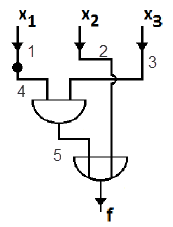
\includegraphics[width=3cm]{images/circuit.png} \hspace{1.5cm}
\begin{tabular}{ll}
$f_1,\dots,f_5$ are 0-jams & $f_6,\dots,f_a$ are 1-jams.\\\hline
 $f_1(x_1,x_2,x_3) = \bar 0x_3+x_2 = x_3+x_2$ & $f_6(x_1,x_2,x_3) = \bar 1x_3+x_2 = x_2$ \\
 $f_2(x_1,x_2,x_3) = \bar x_1x_3+0 = \bar x_1x_3$ & $f_7(x_1,x_2,x_3) = \bar x_1x_3+1 = 1$ \\
 $f_3(x_1,x_2,x_3) = \bar x_10+x_2 = x_2$ & $f_8(x_1,x_2,x_3) = \bar x_11+x_2 = \bar x_1+x_2$ \\
 $f_4(x_1,x_2,x_3) =  0x_3+x_2 = x_2$ & $f_9(x_1,x_2,x_3) =  1x_3+x_2 = x_3+x_2$ \\
 $f_5(x_1,x_2,x_3) = 0+x_2 = x_2$ & $f_a(x_1,x_2,x_3) = 1+x_2 = 1$ \\
\end{tabular}

\vspace{1cm}

Ausfalltafel:
\begin{tabular}{|l||lll||l|l|l|l|l|l|l|l|l|l||l|}\hline
\# & $x_1$&$x_2$&$x_3$&$f_1$&$f_2$&$f_3$&$f_4$&$f_5$&$f_6$&$f_7$&$f_8$&$f_9$&$f_a$&$f$ \\\hline\hline
0  & 0&0&0            & 0   & 0   & 0   & 0   & 0   & 0   & 1   & 1   & 0   & 1   & 0  \\
1  & 0&0&1            & 1   & 1   & 0   & 0   & 0   & 0   & 1   & 1   & 1   & 1   & 1  \\
2  & 0&1&0            & 1   & 0   & 1   & 1   & 1   & 1   & 1   & 1   & 1   & 1   & 1  \\
3  & 0&1&1            & 1   & 1   & 1   & 1   & 1   & 1   & 1   & 1   & 1   & 1   & 1  \\
4  & 1&0&0            & 0   & 0   & 0   & 0   & 0   & 0   & 1   & 0   & 0   & 1   & 0  \\
5  & 1&0&1            & 1   & 0   & 0   & 0   & 0   & 0   & 1   & 0   & 1   & 1   & 0  \\
6  & 1&1&0            & 1   & 0   & 1   & 1   & 1   & 1   & 1   & 1   & 1   & 1   & 1  \\
7  & 1&1&1            & 1   & 0   & 1   & 1   & 1   & 1   & 1   & 1   & 1   & 1   & 1  \\\hline
\end{tabular}

$\Longrightarrow f_1=f_9 ; f_2 ; f_3=f_4=f_5=f_6 ; f_7=f_a ; f_8$

Ausfallmatrix:
\begin{tabular}{|l||lll||l|l|l|l|l||l|}\hline
\# & $x_1$&$x_2$&$x_3$&$f_1$&$f_2$&$f_3$&$f_7$&$f_8$&$f$ \\\hline\hline
0  & 0&0&0            & 0   & 0   & 0   & 1   & 1   & 0  \\
1  & 0&0&1            & 1   & 1   & 0   & 1   & 1   & 1  \\
2  & 0&1&0            & 1   & 0   & 1   & 1   & 1   & 1  \\
3  & 0&1&1            & 1   & 1   & 1   & 1   & 1   & 1  \\
4  & 1&0&0            & 0   & 0   & 0   & 1   & 0   & 0  \\
5  & 1&0&1            & 1   & 0   & 0   & 1   & 0   & 0  \\
6  & 1&1&0            & 1   & 0   & 1   & 1   & 1   & 1  \\
7  & 1&1&1            & 1   & 0   & 1   & 1   & 1   & 1  \\\hline
\end{tabular}

Fehlermatrix:
\begin{tabular}{|l||lll||l|l|l|l|l||l|}\hline
\# & $x_1$&$x_2$&$x_3$&$f\nleftrightarrow f_1$&$f\nleftrightarrow f_2$&$f\nleftrightarrow f_3$&$f\nleftrightarrow f_7$&$f\nleftrightarrow f_8$ & Test\\\hline\hline
0  & 0&0&0            & 0   & 0   & 0   & 1   & 1 & $\star$ \\
1  & 0&0&1            & 0   & 0   & 1   & 0   & 0 & $\star$ \\
2  & 0&1&0            & 0   & 1   & 0   & 0   & 0 & $\star$ \\
3  & 0&1&1            & 0   & 0   & 0   & 0   & 0 & \\
4  & 1&0&0            & 0   & 0   & 0   & 1   & 0 & \\
5  & 1&0&1            & 1   & 0   & 0   & 1   & 0 & $\star$ \\
6  & 1&1&0            & 0   & 1   & 0   & 0   & 0 & \\
7  & 1&1&1            & 0   & 1   & 0   & 0   & 0 & \\\hline
\end{tabular}

$\Longrightarrow$ Testvector: $\{(0,0,0),(0,0,1),(0,1,0),(1,0,1)\}$


\FloatBarrier
\section*{Exercise 5.2 (Row and Column-Rules are not a function)}
todo

\FloatBarrier
\section*{Exercise 6.3 (Hazards)}

%Dummy table please leave it here

\begin{tabular}{|c||c|c|c|c|}
  \hline
  \multicolumn{5}{|c|}{$x_1=1$} \\ \hline
            & \multicolumn{4}{c|}{$x_4x_5$} \\
$x_2x_3$ & 00                  & 01                  & 11                 & 10                  \\ \hline\hline
    00   &                     & \cellcolor{green}1  &                    &                     \\ \hline
    01   &                     & \cellcolor{green}1  &                    & \cellcolor{magenta}1\\ \hline
    11   & \cellcolor{red}1    & \cellcolor{yellow}1 &                    & \cellcolor{magenta}1\\ \hline
    10   & \cellcolor{red}1    & \cellcolor{yellow}1 &                    &                     \\
  \hline
\end{tabular}\\[5mm]
which yields: $f   =  \textcolor{blue}{\neg x_1x_2\neg x_3\neg x_4}+
                      \textcolor{orange}{\neg x_1\neg x_2\neg x_3\neg x_5}+
                      \neg x_1x_2x_3x_4x_5+
                      \textcolor{red}{x_1x_2\neg x_4}+
                      \textcolor{green}{x_1\neg x_4x_5}+
                      \textcolor{magenta}{x_1x_3x_4\neg x_5}$\\

\end{document}
